\newpage
\usecasegenerico{Ricerca di ristoranti}
\label{usecase:Ricerca di ristoranti}

\begin{figure}[h]
	\centering
	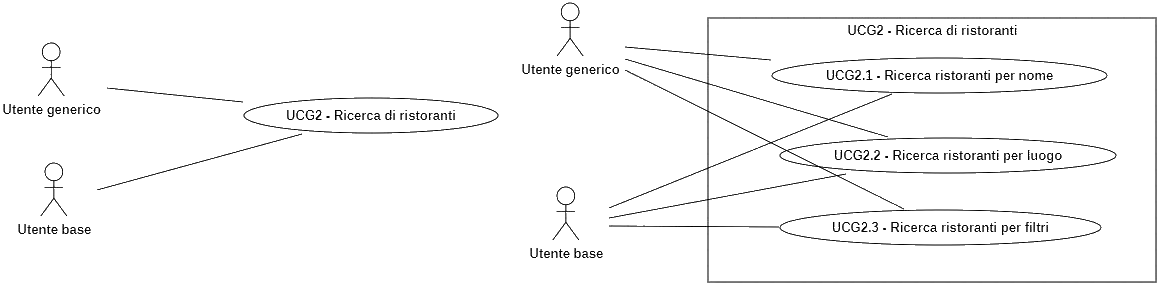
\includegraphics[width=0.99\textwidth]{./uml/UCG2.png} 
	\caption{Ricerca di ristoranti}
	\label{fig:UCG2}
\end{figure}

\begin{itemize}
	\item \textbf{Attori principali:} 
	\begin{itemize}
		\item Utente generico.
		\item Utente base.
	\end{itemize}

	\item \textbf{Precondizione:}
	      L'utente è connesso al Sistema.

	\item \textbf{Postcondizione:} L'Attore principale ricerca dei ristoranti secondo tre modalità: per nome, per luogo, applicando dei filtri.

	\item \textbf{Scenario principale:}
	      \begin{enumerate}
		      \item Il Sistema presenta all'Attore principale tre modalità di ricerca dei ristoranti:
		            \begin{itemize}
			            \item Possibilità di ricercare il ristorante per nome (vedi \autoref{usecase:Ricerca ristoranti per nome}).
			            \item Possibilità di ricercare il ristorante per luogo (vedi \autoref{usecase:Ricerca ristoranti per luogo}).
			            \item Possibilità di ricercare il ristorante attraverso l'applicazione di filtri (vedi \autoref{usecase:Ricerca ristoranti per filtri}).
		            \end{itemize}

		      \item Il Sistema mostra l'elenco dei ristoranti in base alla modalità selezionata dall'Attore principale (vedi \autoref{usecase:Visualizzazione elenco ristoranti}).

	      \end{enumerate}
\end{itemize}


\subusecasegenerico{Ricerca ristoranti per nome}
\label{usecase:Ricerca ristoranti per nome}
\begin{itemize}
	\item \textbf{Attori principali:} 
	\begin{itemize}
		\item Utente generico.
		\item Utente base.
	\end{itemize}

	\item \textbf{Precondizione:} L'utente è connesso al Sistema.

	\item \textbf{Postcondizione:} Il Sistema mostra l'elenco dei ristoranti secondo la ricerca per nome fatta dall'Attore principale.

	\item \textbf{Scenario principale:}
	      \begin{enumerate}
		      \item L'Attore principale esegue una ricerca del ristorante in base al nome;
		      \item Il Sistema mostra il risultato della ricerca all'Attore principale.
	      \end{enumerate}
\end{itemize}

\subusecasegenerico{Ricerca ristoranti per luogo}
\label{usecase:Ricerca ristoranti per luogo}
\begin{itemize}
	\item \textbf{Attori principali:} 
	\begin{itemize}
		\item Utente generico.
		\item Utente base.
	\end{itemize}

	\item \textbf{Precondizione:} L'utente è connesso al Sistema.

	\item \textbf{Postcondizione:} Il Sistema mostra l'elenco dei ristoranti secondo la ricerca per luogo fatta dall'Attore principale.

	\item \textbf{Scenario principale:}
	      \begin{enumerate}
		      \item L'Attore principale esegue una ricerca del ristorante in base al luogo;
		      \item Il Sistema mostra il risultato della ricerca all'Attore principale.
	      \end{enumerate}
\end{itemize}


\subusecasegenerico{Ricerca ristoranti per filtri}
\label{usecase:Ricerca ristoranti per filtri}
\begin{itemize}
	\item \textbf{Attori principali:} 
	\begin{itemize}
		\item Utente generico.
		\item Utente base.
	\end{itemize}

	\item \textbf{Precondizione:} L'utente è connesso al Sistema.

	\item \textbf{Postcondizione:} Il Sistema mostra l'elenco dei ristoranti secondo la ricerca basata sui filtri applicati dall'Attore principale.

	\item \textbf{Scenario principale:}
	      \begin{enumerate}
		      \item L'Attore principale esegue una ricerca del ristorante in base all'applicazione di uno o più dei seguenti filtri:
		            \begin{itemize}
			            \item Orario.
			            \item Voto.
			            \item Cucina.
			            \item Prezzo.
			            \item Accessibilità per persone con ridotta mobilità.
			            \item Adatto a bambini.
		            \end{itemize}
		      \item Il Sistema mostra il risultato della ricerca all'Attore principale.
	      \end{enumerate}
\end{itemize}
